\documentclass{beamer}\usepackage[]{graphicx}\usepackage[]{color}
%% maxwidth is the original width if it is less than linewidth
%% otherwise use linewidth (to make sure the graphics do not exceed the margin)
\makeatletter
\def\maxwidth{ %
  \ifdim\Gin@nat@width>\linewidth
    \linewidth
  \else
    \Gin@nat@width
  \fi
}
\makeatother

\definecolor{fgcolor}{rgb}{0.345, 0.345, 0.345}
\newcommand{\hlnum}[1]{\textcolor[rgb]{0.686,0.059,0.569}{#1}}%
\newcommand{\hlstr}[1]{\textcolor[rgb]{0.192,0.494,0.8}{#1}}%
\newcommand{\hlcom}[1]{\textcolor[rgb]{0.678,0.584,0.686}{\textit{#1}}}%
\newcommand{\hlopt}[1]{\textcolor[rgb]{0,0,0}{#1}}%
\newcommand{\hlstd}[1]{\textcolor[rgb]{0.345,0.345,0.345}{#1}}%
\newcommand{\hlkwa}[1]{\textcolor[rgb]{0.161,0.373,0.58}{\textbf{#1}}}%
\newcommand{\hlkwb}[1]{\textcolor[rgb]{0.69,0.353,0.396}{#1}}%
\newcommand{\hlkwc}[1]{\textcolor[rgb]{0.333,0.667,0.333}{#1}}%
\newcommand{\hlkwd}[1]{\textcolor[rgb]{0.737,0.353,0.396}{\textbf{#1}}}%

\usepackage{framed}
\makeatletter
\newenvironment{kframe}{%
 \def\at@end@of@kframe{}%
 \ifinner\ifhmode%
  \def\at@end@of@kframe{\end{minipage}}%
  \begin{minipage}{\columnwidth}%
 \fi\fi%
 \def\FrameCommand##1{\hskip\@totalleftmargin \hskip-\fboxsep
 \colorbox{shadecolor}{##1}\hskip-\fboxsep
     % There is no \\@totalrightmargin, so:
     \hskip-\linewidth \hskip-\@totalleftmargin \hskip\columnwidth}%
 \MakeFramed {\advance\hsize-\width
   \@totalleftmargin\z@ \linewidth\hsize
   \@setminipage}}%
 {\par\unskip\endMakeFramed%
 \at@end@of@kframe}
\makeatother

\definecolor{shadecolor}{rgb}{.97, .97, .97}
\definecolor{messagecolor}{rgb}{0, 0, 0}
\definecolor{warningcolor}{rgb}{1, 0, 1}
\definecolor{errorcolor}{rgb}{1, 0, 0}
\newenvironment{knitrout}{}{} % an empty environment to be redefined in TeX

\usepackage{alltt} 
% \usepackage{graphicx}
\usepackage{graphics}
\usepackage[T1]{fontenc}
\usepackage{hyperref}
\usepackage{verbatim}
\setbeamercovered{transparent}
\renewcommand{\ni}{\noindent}
\hypersetup{
  colorlinks   = true, %Colours links instead of ugly boxes
  urlcolor     = blue, %Colour for external hyperlinks
  linkcolor    = blue, %Colour of internal links
  citecolor   = red %Colour of citations
}
%% to include page numbers manually include the next three lines
% \usepackage{fancyhdr,lastpage}
% \pagestyle{fancy}\fancyhf{}\rfoot{\vspace{-0.5cm} Page {\thepage} of \pageref{LastPage}}
% \renewcommand\headrulewidth{0pt} % Removes funny header line
%load packages that will be invisible on slides





\title[Dynamic Documents with knitr]{Dynamic Documents with knitr}
\date{April 9, 2014}
\institute[ISU]{Iowa State University}
\IfFileExists{upquote.sty}{\usepackage{upquote}}{}
\begin{document}
%---------------------------------------------------------------------------

\begin{frame}
    \maketitle
\end{frame}

%---------------------------------------------------------------------------

\begin{frame}
\frametitle{knit what?}
\begin{itemize}
\item Adds (knits) R code into your document so that all of the files for a particular experiment are in one place\medskip
\item Compiling the document also runs the R code, so one button press runs your statistical analysis and places it into your document\medskip
\item Integrates R output with the document text so that pictures, tables, and numeric data are all dependent on the R code\medskip
\item Produces beautiful, seamless  integration of statistical analysis with scientific writing
\end{itemize}
\end{frame}

%---------------------------------------------------------------------------

\begin{frame}
\frametitle{Reproduceable Research}
\begin{itemize}
\item Journals often require code and data to be included in a paper submission so the analysis can be reproduced\medskip
\item Statistical analyses are often re-used for multiple similar experiments\medskip
\item We don't always comment code when we write it - knitr provides context for the code by including the writeup with the code
\end{itemize}
\end{frame}

%---------------------------------------------------------------------------

\begin{frame}
\frametitle{Setup}
\begin{itemize}
\item LaTeX: If you don't have this installed, you will need to use our computers.\medskip
\item knitr: use \texttt{install.packages("knitr")} to install the knitr package in R\medskip
\item RStudio: \\{\footnotesize Tools $-\!\!\!>$ Global Options $-\!\!\!>$ Sweave $-\!\!\!>$ Weave Rnw files using knitr}\\ (This tells RStudio to use knitr to compile the document)
\end{itemize}
\end{frame}

%---------------------------------------------------------------------------

\begin{frame}
\frametitle{Example}
Open \href{../code/minimal-knitr.Rnw}{minimal-knitr.Rnw} in RStudio and compile it\\\bigskip
Hint: use the "Compile PDF" button at the top of the text window in RStudio\\\bigskip
\begin{figure}
\centering
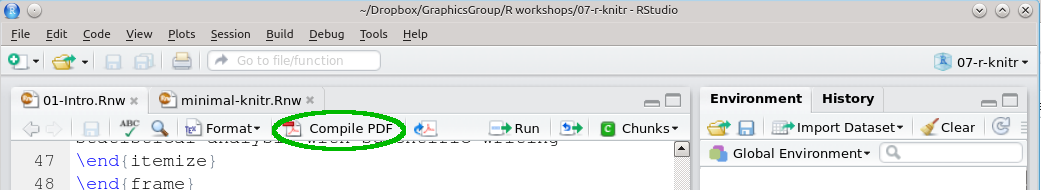
\includegraphics[keepaspectratio=T,width=\textwidth]{figure/compilePdfRstudio}
\end{figure}
\end{frame}

%---------------------------------------------------------------------------

\begin{frame}
\frametitle{R Code "Chunks"}
knitr knows that text is R code if it is included in a "chunk": \bigskip\bigskip

\texttt{<<chunk-label, options=...>>=}\\
\hspace{10pt}\\
\hspace{30pt}\texttt{your code goes here}\\
\hspace{10pt}\\
\texttt{@}\\

\end{frame}

%---------------------------------------------------------------------------

\begin{frame}
\frametitle{Your Turn}
Change \href{../code/minimal-knitr.Rnw}{minimal-knitr.Rnw} so that the second code chunk (named 'boring-random') generates 30 random numbers and computes their sum. \bigskip

Make sure the code chunk compiles!
\end{frame}

%---------------------------------------------------------------------------

\begin{frame}[fragile]
\frametitle{Adding graphs to documents with knitr}
\begin{verbatim}
\centering
<<chunk-label, options=...>>=

      make a plot here

@
\end{verbatim}
\end{frame}

%---------------------------------------------------------------------------

\begin{frame}[fragile]
\frametitle{Your Turn}
Add a new code chunk to \href{../code/minimal-knitr.Rnw}{minimal-knitr.Rnw} that generates a sample of 50 observations from a normal distribution and plot a histogram. 

\begin{knitrout}\footnotesize
\definecolor{shadecolor}{rgb}{1, 1, 1}\color{fgcolor}\begin{kframe}
\begin{alltt}
\hlstd{x} \hlkwb{<-} \hlkwd{rnorm}\hlstd{(}\hlnum{50}\hlstd{)}

\hlkwd{library}\hlstd{(ggplot2)}
\hlkwd{qplot}\hlstd{(x,} \hlkwc{geom}\hlstd{=}\hlstr{"histogram"}\hlstd{)}
\end{alltt}
\end{kframe}
\end{knitrout}


Make sure the code chunk compiles!
\end{frame}

%---------------------------------------------------------------------------

\begin{frame}
\frametitle{knitr code chunk options}
We may want to remove the messages (the italic text) from our R output in the pdf. Or, we might not want to show the code at all. \bigskip\bigskip

knitr has options to give you greater control over what is shown in the compiled document. \bigskip\bigskip

Let's look at these options \href{http://yihui.name/knitr/options}{in the documentation}.
\end{frame}

%---------------------------------------------------------------------------

\begin{frame}[fragile]
\frametitle{knitr code chunk options}
\begin{itemize}
\item \texttt{eval=FALSE}: don't run the code
\item \texttt{echo=FALSE}: don't show the code\bigskip
\item \texttt{warning=FALSE}: don't add R's warnings to the pdf
\item \texttt{message=FALSE}: don't show messages from R in the pdf\bigskip
\item \texttt{include=FALSE}: don't include any R output in the document\\
Pictures are still saved and can be included with \verb|\includegraphics{}|.
\item \texttt{tidy=FALSE}: don't tidy code or change spacing
\item \texttt{cache=FALSE}: re-run all of the code every time.
% \item \texttt{size='normalsize'}: change the latex size of the text output\\
% Can be any valid latex size, from \verb|\Huge| to \verb|\tiny|
\end{itemize}
\end{frame}

%---------------------------------------------------------------------------

\begin{frame}
\frametitle{Your Turn}
Explore some of the options in knitr code chunks. 
\begin{itemize}
\item Turn off messages and warnings for the histogram we generated last time
\item Experiment with \texttt{tidy=TRUE} - what changes occur?
\item Can you make knitr show only the plot, without code, messages, errors, etc.?
\end{itemize}
\end{frame}

%---------------------------------------------------------------------------

\begin{frame}
\frametitle{Common Options for Pictures}
\begin{itemize}
\item \texttt{fig.width=7, fig.height=7}: dimensions of the saved image
\item \texttt{out.width=`\textbackslash\textbackslash textwidth', out.height=`300px'}: dimensions of the image in the LaTeX document. \\ Note: \textbackslash\textbackslash must be used to generate a single slash in LaTeX. \bigskip

\item \texttt{fig.path="path/to/save/figures"}: Change where figures are stored
\item \texttt{dpi=72}: resolution of the saved image\bigskip

\item \texttt{fig.keep=``all"}: Which figures to keep\\
Options: `high', `none', `all', `first', `last'
\item \texttt{fig.show=``asis''}: how to arrange plots\\
Options: `asis', `hold', `animate', `hide'\bigskip
\end{itemize}
\end{frame}

%---------------------------------------------------------------------------

\begin{frame}[fragile]
\frametitle{Your Turn}
\begin{itemize}
\item Generate both a histogram and a density plot in the same code chunk\\
try different \texttt{fig.keep} and \texttt{fig.show} options
\item Change the size of both plots so they will fit on the same page\\
Hint: use \texttt{out.width=``.48\textbackslash\textbackslash textwidth''}
\item Use \texttt{include=FALSE} and include the figure in LaTeX directly:\\
\begin{verbatim}
\begin{figure}[h]\centering
\includegraphics[width=.5\linewidth]
    {figure/codechunkname}
\end{figure}
\end{verbatim}
\end{itemize}
\end{frame}

%---------------------------------------------------------------------------

\begin{frame}[fragile]
\frametitle{More Common Options for Pictures}
\begin{itemize}
\item \texttt{fig.cap="caption text"}: Text for figure caption
\item \texttt{fig.align="center"}: Alignment of the figure on the document page.\\ Options `left', `right', `center'
\item \texttt{fig.pos="htbp"}: Latex positioning options - "h" for here, "t" for top, "b" for bottom, "p" a page of floats. 
\item \texttt{fig.env=}: LaTeX environment for figures (i.e. SCfigure, marginfigure)
\item \texttt{fig.lp="fig:"}: Label prefix for figure label: the actual label will concatenate this prefix and the chunk label. So to reference a figure in chunk ``plot" in a LaTeX paragraph, you would use \verb|\ref{fig:plot}| to get the plot number. 
\end{itemize}
\end{frame}

%---------------------------------------------------------------------------

\begin{frame}[fragile]
\frametitle{Setting commonly used options for all chunks}
It is common to create a setup chunk at the beginning of a LaTeX document (i.e. before the \textbackslash begin\{document\} line) to load packages and set default options. 

\begin{verbatim}
<<setup,cache=FALSE,echo=FALSE>>=

opts_chunk$set(fig.width=6, fig.height=6, tidy=FALSE, echo=FALSE)

@
\end{verbatim}
\end{frame}

%---------------------------------------------------------------------------

\begin{frame}
\frametitle{Your Turn}

Try setting default options at the beginning of our Rnw file, and see how things change. \bigskip\bigskip

Notice that you can always override default options within each chunk header.

\end{frame}

%---------------------------------------------------------------------------

\end{document}
